\documentclass{article}

% Language setting
\usepackage[english]{babel}

% Set page size and margins
\usepackage[a4paper,top=2cm,bottom=2cm,left=3cm,right=3cm,marginparwidth=1.75cm]{geometry}
% Useful packages
\usepackage{amsmath}
\usepackage{graphicx}
\usepackage[colorlinks=true, allcolors=black]{hyperref}
\usepackage{listings}
\usepackage{xcolor}

\definecolor{codegreen}{rgb}{0,0.6,0}
\definecolor{codegray}{rgb}{0.5,0.5,0.5}
\definecolor{codepurple}{rgb}{0.58,0,0.82}
\definecolor{backcolour}{rgb}{0.95,0.95,0.92}

\lstdefinestyle{mystyle}{
    backgroundcolor=\color{backcolour},   
    commentstyle=\color{codegreen},
    keywordstyle=\color{magenta},
    numberstyle=\tiny\color{codegray},
    stringstyle=\color{codepurple},
    basicstyle=\ttfamily\footnotesize,
    breakatwhitespace=false,         
    breaklines=true,                 
    captionpos=b,                    
    keepspaces=true,                 
    numbers=left,                    
    numbersep=5pt,                  
    showspaces=false,                
    showstringspaces=false,
    showtabs=false,                  
    tabsize=2
}

\lstset{style=mystyle}

\title{Haskell Project}
\author{Jan Lucca Thümmel - jathu21@student.sdu.dk}

\begin{document}
\maketitle


\tableofcontents
\newpage

\section{Introduction}
The goal of the project is to draw fractals using L-Systems and turtle graphics in Haskell. By solving three specific tasks. These task are applying rules to a state, going to target depth and processing a fractal

\section{Specification}

\subsection{Task 1: Applying Rules to a State}
Task 1 is solved by implementing the apply function. The apply function takes a state and a list of rules and returns a state. A state is defined by a list of characters. A rule is defined by a character and a state. The apply function takes a state and rules, checking whether a character in the state has a specific rule. If a character has no rule the next character is checked. When a character has a rule the character gets replaced with the state of the rule. As an example, we have the rules: ’X’ "XRYF", ’Y’ "FXLY" and the state "FXRYF". In this case the apply function would replace every X with "XRYF" and every Y with "FXLY" resulting in the string "FXRYFRFXLYF".

\subsection{Task 2: Going to Target Depth}
Task 2 is solved by implementing the function expand. The expand function takes a state, a list of rules, a target depth in form of an integer and returns a state. The function will apply the apply function to the state until reaching the target depth and then return the result state. An example could be applying these rules: ’X’ "XRYF", ’Y’ "FXLY" to the state "FX" with depth two. Depth one is achieved by applying apply once, giving the string "FXRYF". Depth two is achieved by applying apply again on the new string. Resulting in the new string "FXRYFRFXLYF". This can be repeated until the target depth is reached.

\subsection{Task 3: Processing a Fractal}
Task 3 is solved by implementing the function process. The process function takes a fractal and produces a list of commands to draw the fractal. This is achieved by using the expand function to get the state at target depth. Then the turtle graphics commands are mapped to the state. The commands are produced by the charToCom function which converts a character to a turtle command. Testing the function with the main command in GHCI should produce a white on black snowflake. A picture of the produced snowflake and all other fractals is included in the appendix (section \ref{Fractals}).

\section{Design}
We have some predefined data types that are used by the functions apply, expand and process.

\begin{lstlisting}[language=Haskell]

-- state represented by list of letters
type State = [Char]

-- rule represented by a letter (left-hand side) and a state (right-hand side)
data Rule = Rule Char State deriving Show

-- turtle graphics commands (Nop is no operation)
data Command = Forward | LeftTurn Int | RightTurn Int | Nop | Scale Double | Backward deriving Show 

-- fractal represented by initial state, list of rules, mapping from letters to commands, target depth, initial length
type Fractal = (State, [Rule], Char -> Command, Int, Double)
\end{lstlisting}

We have a state which is simply defined as a list of characters. We have a Rule which consists of a Rule, a Character and a state. We also have Command which consists of turtle graphics commands. The turtle graphics commands are actions the turtle can take when drawing a fractal. They consist of forward, to move forward, LeftTurn Int to turn left with specific degrees, the same is true for RightTurn, Nop for no operation, Scale for scaling and backwards to move backwards. We have a Fractal which consists of an initial state, a list of rules, a function Char $\rightarrow$ Command that maps each character to a turtle graphics command, an int for the desired depth and a Double for the initial length.


\subsection{Task 1: Design}
The goal of the apply function is to apply rules to at state. Apply takes State and rule as input and returns a new State. Apply goes through the initial state and applies the first applicable rule. Characters that have no rule are just copied to the new state. This then gives a new state. Apply thus transforms the state from depth n to depth n+1.
 
\subsection{Task 2: Design}
The goal of the expand function is using apply to go to depth n. The expand function takes an initial state, a list of rules and a target depth. Using recursion the apply function is applied until the target depth is reached.

\subsection{Task 3: Design}
The goal of the process function is to take a fractal description and translate it to turtle graphics commands. Process uses the expand function to get the final state then it maps the function charToCom to the final state to produce the turtle graphics commands.

\section{Implementation}

\subsection{Task 1: Implementation}
\begin{lstlisting}[language=Haskell]
-- go from depth n to depth n+1
apply :: State -> [Rule] -> State
apply state rule = concatMap (replace rule) state  

replace :: [Rule] -> Char -> State
replace [] c = [c]
replace (Rule rc rs:xs) char = if rc == char
    then rs
    else replace xs char
\end{lstlisting}
The apply function is designed, so that it takes a state and a list of rules as input and returns a state. The result state is produced by mapping the replace function over each character in the state. For that a concatMap is used as the result should be a single list. The replace function is a helper function for the apply function. It has the logic for applying the rules. If there are no rules to apply the character stays the same. If the rule character (rc) matches with the character (char) we replace it with the state from the rule. Otherwise we recursively call the replace function again on the remaining rules(xs). 

\subsection{Task 2: Implementation}
\begin{lstlisting}[language=Haskell]
-- expand to target depth
expand :: State -> [Rule] -> Int -> State
expand state rule 0 = state
expand state rule d = expand (apply state rule) rule (d-1)
\end{lstlisting}
The expand function takes  an initial state a list of rules and a target depth. Using recursion it applies the apply function until the target depth is reached. "expand state rule 0 = state" is the base case. If the target depth is zero we just return the current state as the state is unchanged. If the depth is greater than zero expand looks like this "expand state rule d = expand (apply state rule) rule (d-1)". Because this is a recursive implementation the expand function is called until the depth reaches zero and there by achieving the base case, returning the final state with depth n.

\newpage
\subsection{Task 3: Implementation}
\begin{lstlisting}[language=Haskell]
-- convert fractal into sequence of turtle graphics commands
process :: Fractal -> [Command]
process (state, rule, charToCom, depth, scale) =  
    let finalState = expand state rule depth
    in map charToCom finalState

charToCom :: Char -> Int -> Command
charToCom 'F' _ = Forward 
charToCom 'L' turn = LeftTurn turn
charToCom 'R' turn = RightTurn turn
charToCom 'B' _ = Backward
charToCom  _ _ = Nop
\end{lstlisting}
The process function takes a fractal as input. It translates the fractal to turtle graphics commands so the fractal can be drawn. We obtain the final state by using the expand function with the desired depth. Then we map the helper function, charToCom onto the final state to get the commands. The function charToCom uses pattern matching to decide which command should be chosen based on the input character. For example if the character is F the function chooses Forward. If a character doesn't match the predefined commands it gets matched with Nop(no operation). This is done by the two underscores. Which represent any other input that is not defined.

\section{Testing}
The implementation was tested by testing the functions apply, expand and process. The apply function was tested by this command in GHCI: "apply "FXRYF" [Rule ’X’ "XRYF", Rule ’Y’ "FXLY"]", and then checking if the function returned the desired out put. Which in this case would be "FXRYFRFXLYF". The expand function was tested in a similar way by using this command: "expand "FX" [Rule ’X’ "XRYF", Rule ’Y’ "FXLY"] 2". The desired output in this case would be "FXRYFRFXLYF". The function process was tested by drawing the different fractals and checking if the output is as desired. This also test apply and expand as these functions, have to be implemented the right way to draw the desired fractals. By looking at the fractals we can see if the implementation is correct. All of the example fractals are provided in the appendix (section \ref{Fractals}).

\section{Conclusion}
The three main tasks of implementing the functions apply, expand and process where implemented successfully. The apply function was successfully implemented to apply rules to a state. This was confirmed by testing the function. The expand function was successfully implemented, with the help of the apply function, to reach the targeted depth. this was done by recursively applying the apply function until the desired depth is reached. The correctness of the implementation was also confirmed by testing. The process function that translates a final state into turtle graphics commands was also successfully implemented with the helper function charToCom. The implementation was also shown to be correct by the program drawing the correct fractals. The three implemented functions thus also work together. The current implementation meets the project requirements but future improvements may include optimizing the code or implementing the support for colours and line width to make the fractals look even better.


\section{Appendix}

\subsection{Fractals} \label{Fractals}

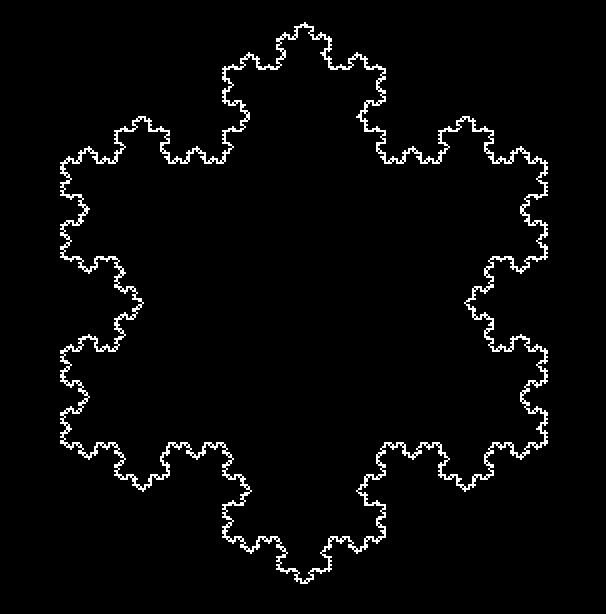
\includegraphics[width=\textwidth]{pictures/snowflake.png}
\newpage
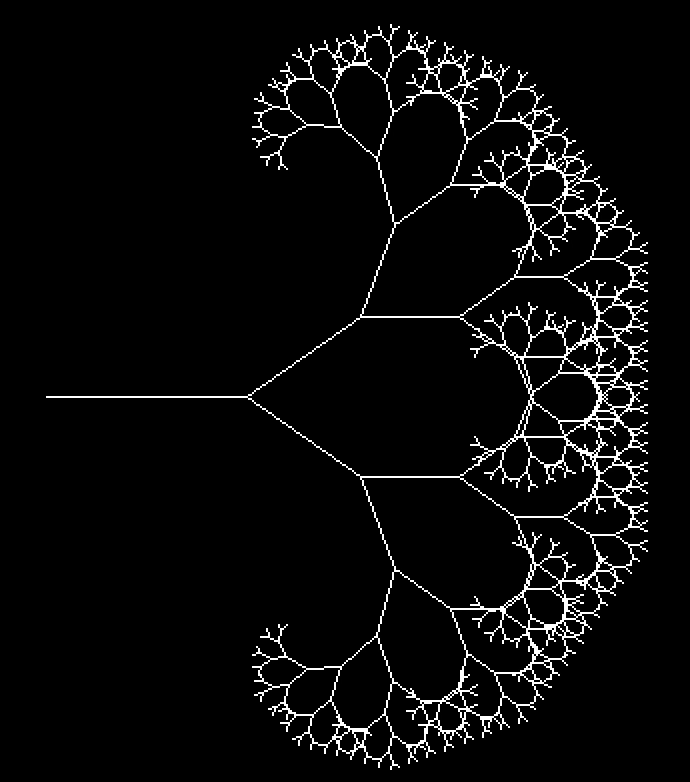
\includegraphics[width=\textwidth]{pictures/tree.png}
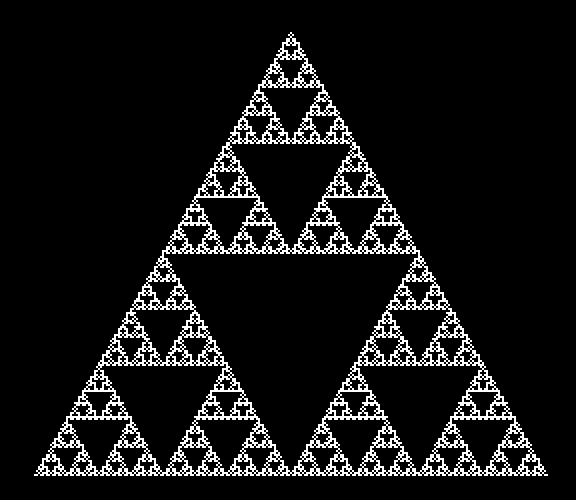
\includegraphics[width=\textwidth]{pictures/sierpinski.png}
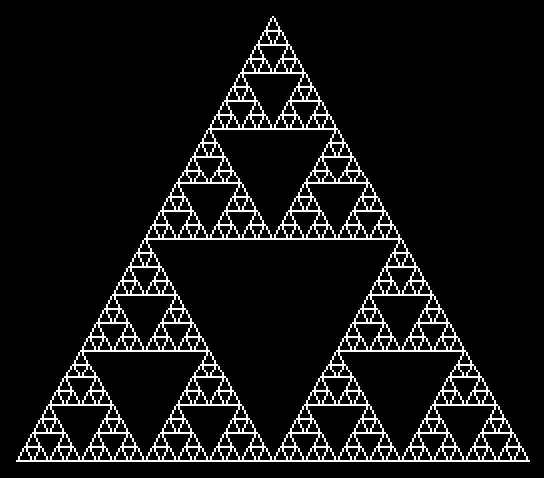
\includegraphics[width=\textwidth]{pictures/sierpinksi2.png}
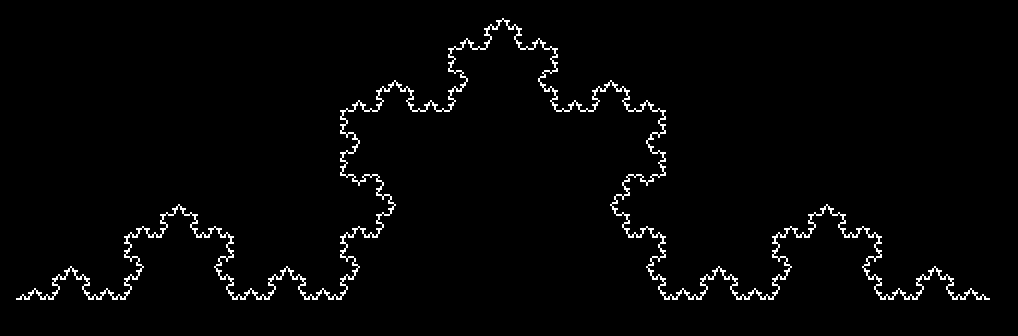
\includegraphics[width=\textwidth]{pictures/koch.png}
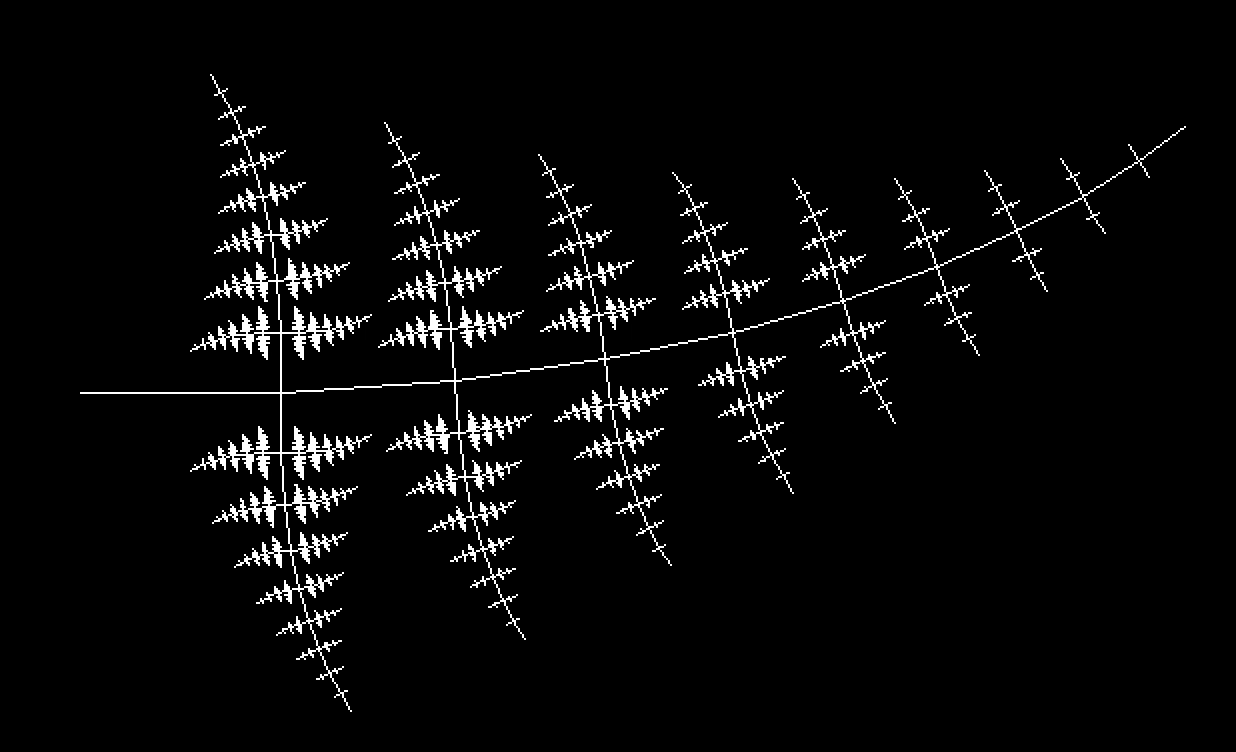
\includegraphics[width=\textwidth]{pictures/fern.png}
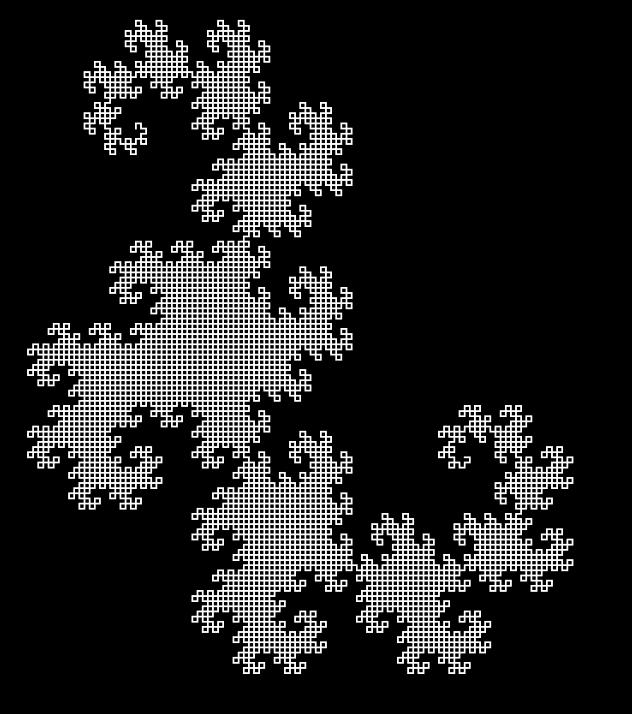
\includegraphics[width=\textwidth]{pictures/dragon.png}


\subsection{Code} \label{Code}
\begin{lstlisting}[language=Haskell]
import Graphics.HGL

-- state represented by list of letters
type State = [Char]

-- rule represented by a letter (left-hand side) and a state (right-hand side)
data Rule = Rule Char State deriving Show

-- turtle graphics commands (Nop is no operation)
data Command = Forward | LeftTurn Int | RightTurn Int | Nop | Scale Double | Backward deriving Show 

-- turtle represented by reference to window, current position, current angle, current length
type Turtle = (Window, Double, Double, Double, Double)

-- fractal represented by initial state, list of rules, mapping from letters to commands, target depth, initial length
type Fractal = (State, [Rule], Char -> Command, Int, Double)

-- examples for rule lists
rules1 = [Rule 'F' "FLFRFLF"]
rules2 = [Rule 'X' "XRYF", Rule 'Y' "FXLY"]

-- examples for fractals
fractal1 = ("F", rules1, let m 'F' = Forward; m 'L' = LeftTurn 60; m 'R' = RightTurn 120 in m)
fractal2 = ("FX", rules2, let m 'F' = Forward; m 'L' = LeftTurn 90; m 'R' = RightTurn 90; m _ = Nop in m)

-- go from depth n to depth n+1
apply :: State -> [Rule] -> State
apply state rule = concatMap (replace rule) state  

replace :: [Rule] -> Char -> State
replace [] c = [c]
replace (Rule rc rs:xs) char = if rc == char
    then rs
    else replace xs char
 
-- expand to target depth
expand :: State -> [Rule] -> Int -> State
expand state rule 0 = state
expand state rule d = expand (apply state rule) rule (d-1)

-- convert fractal into sequence of turtle graphics commands
process :: Fractal -> [Command]
process (state, rule, charToCom, depth, scale) =  
    let finalState = expand state rule depth
    in map charToCom finalState

charToCom :: Char -> Int -> Command
charToCom 'F' _ = Forward 
charToCom 'L' turn = LeftTurn turn
charToCom 'R' turn = RightTurn turn
charToCom 'B' _ = Backward
charToCom  _ _ = Nop

-- helper function to go from two floating point values to a pair of integers
toPoint :: Double -> Double -> Point
toPoint x y = (round x, round y)

-- main turtle graphics drawing function
drawIt :: Turtle -> [Command] -> IO ()
drawIt _                     []                    = return ()
drawIt turtle                (Nop:xs)              = drawIt turtle xs
drawIt (w, x, y, angle, len) (Forward:xs)          = let
  x' = x+len*(cos angle)
  y' = y-len*(sin angle)
  in do
    drawInWindow w (line (toPoint x y) (toPoint x' y'))
    drawIt (w, x', y', angle, len) xs
drawIt (w, x, y, angle, len) (Backward:xs)          = let
  x' = x-len*(cos angle)
  y' = y+len*(sin angle)
  in do
    drawInWindow w (line (toPoint x y) (toPoint x' y'))
    drawIt (w, x', y', angle, len) xs
drawIt (w, x, y, angle, len) (LeftTurn degree:xs)  = let angle' = angle+(fromIntegral degree)*pi/180 in
    drawIt (w, x, y, angle', len) xs
drawIt (w, x, y, angle, len) (RightTurn degree:xs) = let angle' = angle-(fromIntegral degree)*pi/180 in
    drawIt (w, x, y, angle', len) xs
drawIt (w, x, y, angle, len) (Scale factor:xs)     = let len' = len*factor in
    drawIt (w, x, y, angle, len') xs

-- draw a fractal by opening a window and using turtlegraphics
drawFractal fractal@(_, _, _, _, len) = runGraphics (withWindow_ "L-System using Turtle Graphics" (1000, 600)
        (\ w -> do
         drawIt (w, 500, 300, 0, len) (process fractal)
         getKey w))

-- create a list of lists of string, where each list contains the "words" of one line
split :: String -> String -> [String] -> [[String]]
split []        [] []  = []
split ('\n':xs) [] []  = split xs [] []
split ('\n':xs) [] zss = split xs [] []
split ('\n':xs) ys zss = reverse (reverse ys : zss) : split xs [] []
split (' ':xs)  [] zss = split xs [] zss
split (' ':xs)  ys zss = split xs [] (reverse ys:zss)
split (x:xs)    ys zss = split xs (x : ys) zss

-- interpret the list of lists as a description of initial state, rules, mapping, depth, and length of a fractal
interpret :: [[String]] -> State -> [Rule] -> (Char -> Command) -> Int -> Double -> Fractal
interpret []                   start rules m depth len = (start, rules, m, depth, len)
interpret (("rule":xs):yss)    start rules m depth len = interpret yss start (rules ++ [interpretRule xs]) m depth len where
  interpretRule (l:"->":rs) = Rule (head l) (foldr (++) [] rs)
interpret (("start":xs):yss)   _     rules m depth len = interpret yss (foldr (++) [] xs) rules m depth len
interpret (("cmd":xs):yss)     start rules m depth len = interpret yss start rules (interpretCmd xs m) depth len where
  interpretCmd [c, "fd"]            m = \x -> if x == (head c) then Forward else m x
  interpretCmd [c, "lt", deg]       m = \x -> if x == (head c) then LeftTurn (read deg) else m x
  interpretCmd [c, "rt", deg]       m = \x -> if x == (head c) then RightTurn (read deg) else m x
  interpretCmd [c, "nop"]           m = \x -> if x == (head c) then Nop else m x
  interpretCmd [c, "scale", factor] m = \x -> if x == (head c) then Scale (read factor) else m x
  interpretCmd [c, "bk"]            m = \x -> if x == (head c) then Backward else m x
interpret (("length":arg:xs):yss) start rules m depth _   = interpret yss start rules m depth (read arg)
interpret (("depth":arg:xs):yss)  start rules m _     len = interpret yss start rules m (read arg) len

-- read from given file and return a fractal
readFractal fileName = do
  text <- readFile fileName
  return (interpret (split text [] []) [] [] (\x -> error "unknown command") 0 0)

-- daw a fractal described in an .fdl file
drawFdl fileName = do
  fractal <- readFractal fileName
  drawFractal fractal

-- main function that draws the snowflake fractal
main :: IO ()
main = drawFdl "examples/snowflake.fdl"
\end{lstlisting}
\end{document}